\documentclass{scrartcl}

\usepackage{enumitem}
\usepackage{wrapfig}
\usepackage{multicol}
\usepackage{fontspec}
\usepackage{graphicx}
\usepackage{hyperref}
\usepackage[utf8]{inputenc} 
\usepackage[dvipsnames]{xcolor}
\usepackage[textwidth = 17cm, centering]{geometry}
\setmainfont[Ligatures=TeX]{Inkfree.ttf}
\usepackage[spanish]{babel}  
% some colors
\definecolor{fondpaille}{cmyk}{0, 0, 0.1, 0}

\usepackage{sectsty}

\sectionfont{\color{Maroon}\Large\fontspec{Zapfino.ttf}}
\subsectionfont{\color{Maroon}\normalsize\fontspec{Zapfino.ttf}}

\subsubsectionfont{\color{Maroon}\normalsize\fontspec{Zapfino.ttf}}

\newcommand{\msection}[2]{\section{#1}{\color{Maroon}\fontspec{Zapfino.ttf}\begin{center}#2\end{center}}}

\begin{document} 
	\pagecolor{fondpaille}
	\begin{center}
		\scshape
		\color{Maroon}            
		\fontspec{Zapfino.ttf}
		Principios Científicos de la Cocina Molecular
			
		\huge
		Menú Final
		
		\vspace{1cm}
		\footnotesize
		Laura Bellón, Juan Barbosa, Juan Sebastián Bautista,
		
		Michelle Arrighi, Ana Benavides
	\end{center}
	
	\Large
	
	Para el proyecto final, se realizará un menú de tres platos (entrada, plato fuerte y postre) con base en los conocimientos adquiridos a lo largo del semestre y la curiosidad por la cocina molecular. El tema de este menú es la \textbf{“Amazonía, el pulmón del planeta”}, pues se quiere hacer énfasis en el daño que el ser humano le está causando al planeta.  
	
	Por ello, en la entrada se pretende utilizar colores vivos que den alusión y simbolicen la armonía de la selva y todos los seres vivos pertenecientes a esta región, para el plato fuerte, los colores y los componentes de los ingredientes se van a ir opacando, para mostrar la transición del deterioro, por último, para el postre se volverán a revivir los colores vivos utilizados en un comienzo para hacerle la invitación a los comensales de contribuir al cuidado del planeta.  
	
	El escenario simulará una selva, por lo que, estará ambientado con sonidos pertenecientes a este entorno (río) y se proyectarán árboles y animales. Cómo se mencionó anteriormente, se jugará con la diversidad de los colores. En la entrada se colocarán tarros de hielo seco, para simular la neblina de la mañana.
	
	\newpage
	\tableofcontents
	
	\newpage
	\msection{Entrada}{Plátano relleno}
	Son una entrada típica de la región amazónica, al igual que el juane; siendo distinguidos a nivel internacional por su sabor y generosidad, suelen servirse rellenos de alguna proteína bien sea carne de res o camarones y maní. \cite{travel, tipicos}
	\subsection{T\'ecnica}
	La técnica utilizada para la entrada es la cocción por el cambio de pH para los camarones. 
	\subsection{Ingredientes}
	\begin{multicols}{2}
		\begin{itemize}
			\item 1 pl\'atano verde
			\item 50 - 100 g de camarones
			\item 1 lim\'on grande
			\item 50 g de man\'i
		\end{itemize}
	\end{multicols}

	\subsection{Procedimiento}
	\begin{multicols}{2}
		\begin{enumerate}
			\item Lavar el plátano sin pelar, quitarle los extremos, cortarlo en 4-6 pedazos de tamaños iguales y pelarlo.
			\item Hornear por aproximadamente 15 min a una temperatura de 180 $^\circ$C.
			\item Lavar los camarones.
			\item Extraer el zumo de limón y dejar marinar los camarones por 20 min.
			\item Picar el maní en trozos muy pequeños.
			\item Retirar los camarones del zumo de limón y agregarle la sal y pimienta al gusto.
			\item Abrir los trozos de plátano por la mitad y colocar el maní y los camarones en el interior.
		\end{enumerate}
	\end{multicols}
	
	\subsection{Montaje}
		Se hará uso de un plato adornado por medió de hojas de plátano sobre las cuales se servirán los trozos del plátano relleno con el propósito de poder utilizar estas para sujetar los trozos y comerlos sin la necesidad de cubiertos.
	
	\msection{Plato fuerte}{Salm\'on en salsa de a\c{c}a\'i y copoazú}
		El salmón es un alimento sano por su alto contenido en proteínas y ácidos grasos omega-3, por lo cual se han convertido en especies muy valoradas en la pesca. En general, est\'an distribuidos por los océanos y mares de casi todo el mundo, as\'i como r\'ios y lagunas \cite{mills1989ecology}. El a\c{c}a\'i y copoazú constituyen alimentos muy importantes en la dieta amazónica, en donde su cultivo se ha extendido en las \'ultimas d\'ecadas. Crecen en zonas inundables en las riberas de los ríos.  El a\c{c}a\'i se consume en forma de bebidas, dulces, e incluso helados. 
	
	\subsection{T\'ecnica}
		El salm\'on ser\'a cocido usando un horno de convecci\'on, a presi\'on constante y temperatura de 400 $^\circ$F.
	\subsection{Ingredientes}
	\begin{multicols}{2}
		\begin{itemize}
			\item 1 libra de filete de salmón
			\item 25 gr de mantequilla sin sal
			\item 4-5 gr de ajo picado
			\item 1/2 cucharada de cebolla en polvo
			\item 1/2 cucharada de paprika
			\item 1/2 cucharadita de pimienta
			\item albahaca, y sal
			\item 2 cucharadas de jugo de a\c{c}a\'i y copoazú
		\end{itemize}
	\end{multicols}
	
	\subsection{Procedimiento \cite{salmon}}
	\begin{multicols}{2}
		\begin{enumerate}
			\item Colocar una refractaria previamente engrasada con mantequilla en el horno a 400 $^\circ$F.
			
			\item Frotar ambos lados del salmón seco con toallas de papel, y sazonar ambos lados con sal y pimienta.
			
			\item En una sartén pequeña, derretir la mantequilla, y agregar el ajo picado, el pimentón, la cebolla en polvo y la albahaca. Revolver durante unos 30 segundos o 1 minuto. Agregue el jugo de a la mezcla.
			
			\item Adicionar el salm\'on a la refractaria y verter el jugo preparado anteriormente sobre este.
			
			\item Hornear, alrededor de 10-15 minutos.
		\end{enumerate}
	\end{multicols}

	\subsection{Montaje}
	El plato se sirve sobre material alusivo a la \textit{Victoria amazonica}, en donde se busca resaltar el paisaje característico de la región, y su importancia hidrica para el mundo.
	
	\newpage
	\msection{Postre}{Caviar de menta con mojito granizado}
	\subsection{Caviar de menta}
	Para el caviar de menta se utiliza la técnica de esferificación, se trata de una gelificación controlada de un líquido. Surge en un baño para convertirse en esfera. Esta técnica fue empleada por primera vez por los persas al igual que por los romanos, llegándole a atribuir cualidades curativas al caviar. Durante la Edad Media, en Rusia, el caviar se convirtió en un elemento de distinción y buen gusto en las mesas pudientes de occidente, tras la Revolución Rusa de 1917, esto se debió, a la emigración de gran parte de la aristocracia rusa a París en la década de 1920. \cite{davidson2014oxford}
	
	A continuación, se va a utilizar la gelificación de un líquido a través de la esferificación normal, en este caso, se emplea una solución de alginato de sodio y la adición de cloruro cálcico a la mezcla de la menta, se crea una reacción química, de ahí que, el alginato es un polisacárido aniónico presente en las algas marinas pardas y, el cloruro cálcico es un compuesto utilizado para hacer esferificaciones, por lo que, interviene en la creación de bolitas tipo caviar.
	
	\subsubsection{Ingredientes}
		\begin{multicols}{2}
			\begin{itemize}
				\item 225 g agua 
				\item 35 g pasta pura de menta 
				\item 15 g azúcar 
				\item 1,3 g alginato de sodio
				\item 500 g agua 
				\item 2.5 g cloruro cálcico 
			\end{itemize}
		\end{multicols}
	
	\subsubsection{Procedimiento \cite{maite}}
	\begin{multicols}{2}
		\begin{enumerate}
			\item Triturar con la batidora la pasta pura de menta con el alginato.  
			\item Verter en la bandeja inferior de la caviarera y dejar reposar en la nevera para que pierda el aire.
			\begin{center}
				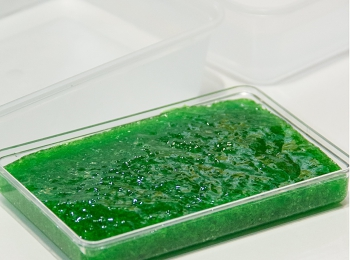
\includegraphics[width = 0.4\textwidth]{images/caviar1}
			\end{center}
		
			\item Mezclando el agua con el cloruro cálcico, se prepara el baño en un recipiente de proporciones similares a la caviarera.
			\begin{center}
				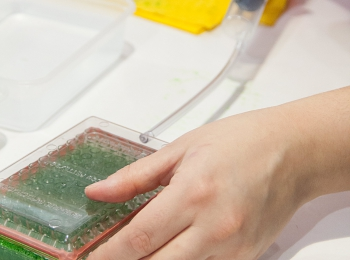
\includegraphics[width = 0.4\textwidth]{images/caviar2}
			\end{center}
		
			\item Con la bandeja de la mezcla de menta y alginato sobre la mesa, se encaja la caviarera y se aspira con la jeringuilla de modo que absorba el líquido.
			\begin{center}
				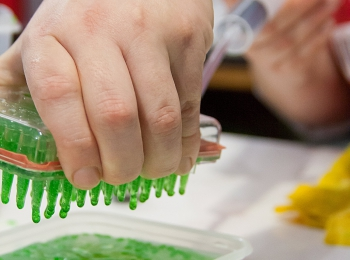
\includegraphics[width = 0.4\textwidth]{images/caviar3}
			\end{center}
		
			\item Pasado este tiempo y con una cuchara coladora, se retiran las esferas y se pasan a dos baños de agua para detener el efecto gelificante y limpiarlas del sabor del cloruro antes de servir.
		\end{enumerate}
	\end{multicols}
	\newpage
		\subsection{Granizado de mojito}
			\subsubsection{Ingredientes}
				\begin{multicols}{2}
					\begin{itemize}
						\item 390 g zumo lima colado 
						\item 90 g azúcar moreno 
						\item 60 g ron negro 
						\item 20 gotas de esencia de lima
					\end{itemize}
				\end{multicols}
			     
			\subsubsection{Procedimiento \cite{maite}}
			\begin{multicols}{2}
				\begin{center}
					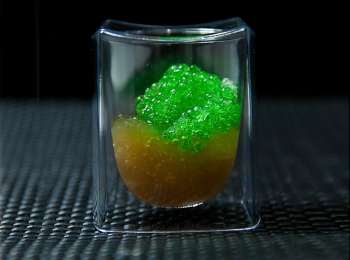
\includegraphics[width = 0.4\textwidth]{images/caviar4}
				\end{center}
				\begin{enumerate}
					\item Se trituran todos los ingredientes con una batidora y se congelan, con el cuidado de ir removiendo de vez en cuando, para que no se convierta en un bloque de hielo. 
					\item Una vez adquiera la textura de granizado, se emplata con un chorro de ron al gusto y el caviar de menta.   
					\item Es importante servir inmediatamente para que ni el caviar ni el granizado pierdan su forma y textura. 
				\end{enumerate}
			\end{multicols}
		
		\subsection{Montaje}
			Para servir el postre, se hace uso de cajas de Petri, de tal manera que, el granizado de mojito quede en la superficie del recipiente y el caviar de menta en la parte de arriba, tal como se muestra en la ilustración, además se colocará un embudo al revés, haciendo parecer que el plato está tapado, generando curiosidad al comensal. 
	
	\newpage
	\bibliography{references}
	\bibliographystyle{unsrt}
\end{document}